\documentclass[12pt]{article}
\usepackage[margin=1in]{geometry}
\usepackage{amsmath,amssymb,amsthm,booktabs,graphicx,natbib,microtype}
\newtheorem{theorem}{Theorem}
\newtheorem{proposition}[theorem]{Proposition}
\newtheorem{remark}[theorem]{Remark}
\title{Robust Overlap Coherence of the Reset Packet Atlas\\\large Principal Angles, Polar Transitions, and a Finite Conditioning Wall}
\author{Prime Dynamics Theory Program}
\date{July 2026}

\begin{document}
\maketitle

\begin{abstract}
RH-151 certified an independent clock-rank top-packet ball at each of 130
source-memory snapshots.  Spectral existence alone does not produce a moving
frame: consecutive exact packet spaces must retain a full-rank overlap after
both endpoint balls are inserted.

Let $U,V$ be nominal orthonormal frames, let
$\alpha=\sigma_{\min}(U^*V)$, and suppose exact projectors lie within radii
$\epsilon_U,\epsilon_V$.  We prove two outward overlap lowers.  The
principal-angle triangle gives
\[
 \widetilde\alpha\geq
 \cos\!\left(\arccos\alpha+arcsin\epsilon_U+arcsin\epsilon_V\right)_+,
\]
while polar-aligned frames give
\[
 \widetilde\alpha\geq
 \left(\alpha-f(\epsilon_U)-f(\epsilon_V)\right)_+,
 \quad f(e)=\sqrt{2-2\sqrt{1-e^2}}.
\]
Their maximum is a valid robust lower.  A positive lower controls both the
inverse overlap and the canonical polar transition; the zero boundary is
sharp because the packet balls can then contain orthogonal subspaces.

All 120 frozen consecutive transitions certify as invertible.  The minimum
robust overlap is $8.9866\times10^{-5}$, the maximum inverse-overlap upper is
$1.1128\times10^4$, and every polar transition is stable with radius below
$0.01170$.  Thus the reset route remains open at finite horizon, but not with
a uniform conditioning constant: 19 transitions are below $0.1$, six below
$0.01$, and two below $0.001$.  The next layer must propagate these actual
condition numbers through the outward Gram/tail assembly.
\end{abstract}

\section{The overlap interface}
For equal-rank orthogonal projectors $P,Q$, the largest principal angle
$\theta_{\max}$ satisfies
\[
 \|P-Q\|=\sin\theta_{\max},\qquad
 \sigma_{\min}(U^*V)=\cos\theta_{\max}
\]
for any orthonormal frames $U,V$ of their ranges.  A transition map is
invertible exactly when $\theta_{\max}<\pi/2$.

RH-151 supplies nominal frames $U_t$ and projector balls
$\|\widetilde P_t-P_t\|\leq\epsilon_t$.  The aim is an outward lower for
$\sigma_{\min}(\widetilde U_{t-1}^*\widetilde U_t)$ independent of frame
signs and internal rotations.

\section{Two robust overlap lowers}
The largest principal angle is a metric on the Grassmannian
\citep{StewartSun1990}.  Therefore
\[
 \widetilde\theta
 \leq\arcsin\epsilon_U+\arccos\alpha+\arcsin\epsilon_V.
\]

\begin{theorem}[Angular overlap lower]\label{thm:angular}
With the notation above, put
\[
 a=\arccos\alpha+\arcsin\epsilon_U+\arcsin\epsilon_V.
\]
If $a<\pi/2$, then every pair of exact packet spaces in the two balls obeys
\[
 \sigma_{\min}(\widetilde U^*\widetilde V)\geq\cos a.
\]
If $a\geq\pi/2$, no positive lower follows from the three scalar data alone.
\end{theorem}
\begin{proof}
The triangle inequality proves the first statement.  At equality, rank-one
lines in a common plane can spend the two ball angles in opposite directions
until the exact lines are orthogonal, proving the information boundary.
\end{proof}

Projector balls also give canonically aligned frames.  If
$\|\widetilde P-P\|\leq e$, polar alignment produces frames satisfying
\[
 \|\widetilde U-U\|\leq
 f(e):=\sqrt{2-2\sqrt{1-e^2}}.
\]

\begin{theorem}[Frame overlap lower]\label{thm:frame}
After independent polar alignment at both endpoints,
\[
 \|\widetilde U^*\widetilde V-U^*V\|
 \leq f(\epsilon_U)+f(\epsilon_V)=:\eta.
\]
Consequently
\[
 \sigma_{\min}(\widetilde U^*\widetilde V)
 \geq(\alpha-\eta)_+.
\]
\end{theorem}
\begin{proof}
Expand the overlap difference into one left-frame and one right-frame term;
both untouched frames have operator norm one.  Singular-value Weyl bounds
give the result \citep{Bhatia1997}.
\end{proof}

We use the maximum of the angular and frame lowers.  Neither dominates in all
geometries, and retaining both costs nothing.

\section{Inverse and polar transition control}
Let $C=U^*V$ and let $R=C(C^*C)^{-1/2}$ be its unitary polar factor.  A robust
overlap lower $\underline\alpha>0$ immediately gives
\[
 \|\widetilde C^{-1}\|\leq\underline\alpha^{-1}.
\]
For the polar factors, a standard perturbation inequality gives
\[
 \|\widetilde R-R\|
 \leq\frac{2\|\widetilde C-C\|}
 {\sigma_{\min}(C)+\sigma_{\min}(\widetilde C)}
 \leq\frac{2\eta}{2\alpha-\eta}
\]
when $\alpha>\eta$ \citep{Li1995}.  Thus overlap invertibility and canonical
frame transport are certified by the same endpoint packet balls.

The inverse factor is the dangerous quantity.  A transition can have a very
stable polar rotation while its overlap is almost singular: the rotation
depends on orientation, whereas inverse amplification depends on the weakest
cosine.

\section{The 120-transition audit}
The audit rebuilds the ten RH-151 reset-frame chains and inserts the archived
projector radii at both endpoints of every consecutive transition.  Table
\ref{tab:counts} summarizes the robust overlap distribution.

\begin{table}[t]
\centering
\begin{tabular}{lrrrrr}
\toprule
threshold & positive & $<10^{-1}$ & $<10^{-2}$ & $<10^{-3}$ & zero\\
\midrule
transitions & 120 & 19 & 6 & 2 & 0\\
\bottomrule
\end{tabular}
\caption{Robust reset-overlap counts.}
\label{tab:counts}
\end{table}

All 120 overlap maps remain invertible.  The median robust lower is $0.90183$.
The minimum, $8.9866\times10^{-5}$, occurs on the first
$\sigma=0.01$ right transition and gives inverse upper $1.1128\times10^4$.
The largest polar-transition radius, $0.011695$, occurs elsewhere, on the
fine left chain.  Hence the worst inverse and worst rotation uncertainty are
distinct mechanisms.

The maximum cumulative chain drawdown
\[
 \sum_t-\log\underline\alpha_t
\]
is $32.015$.  This is finite and far smaller than the direct projective
products rejected in RH-146, but it is not evidence for a uniform asymptotic
lower.

\begin{figure}[t]
\centering
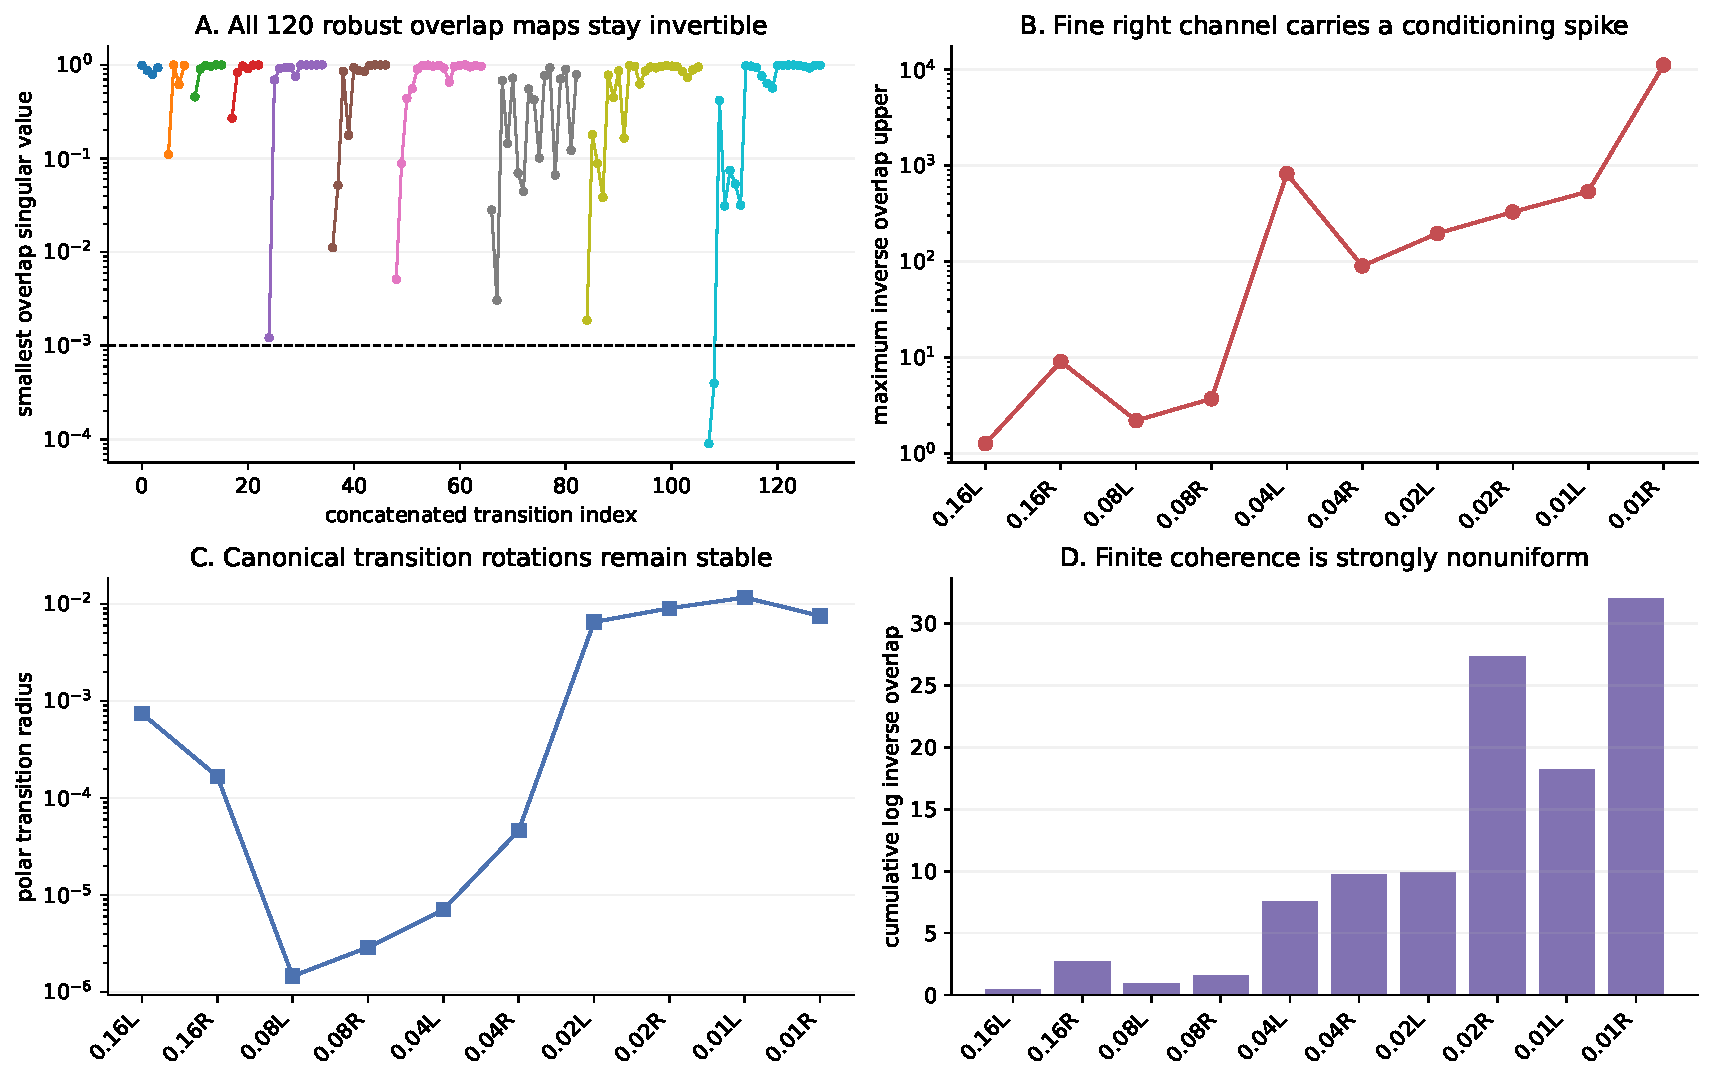
\includegraphics[width=\textwidth]{figures/reset_transition_overlap_coherence.pdf}
\caption{Robust overlaps, inverse amplification, polar radii, and cumulative
conditioning drawdown across the ten reset chains.}
\end{figure}

\section{Consequence and boundary}
The reset atlas is not merely a collection of isolated eigenspaces.  It
supports a finite, canonically aligned moving frame on all five scales and
both channels.  The finite route to an outward assembly therefore remains
open.

What fails is uniform conditioning.  An argument that replaces all overlap
maps by one harmless constant would discard a factor above $10^4$ at a single
birth transition.  RH-153 must derive Gram and tail transport with the
actual transition-by-transition inverse bounds, then determine whether the
large factors are multiplied, canceled, or confined to a finite prefix.

We have not built that outward assembly, proved a uniform overlap lower,
closed the reset source-to-support interface, established Stage A,
constructed a Hilbert--Polya operator, identified zeta zeros, or proved the
Riemann Hypothesis.

\bibliographystyle{plainnat}
\bibliography{references}
\end{document}
